\chapter{Identificação do Túnel de Ar} \label{cap4}

Neste capítulo, será explicada a identificação do sistema do túnel de ar. Para fazer a identificação caixa-preta de um sistema é necessário fazer um estudo prévio do funcionamento dele, conhecer entradas e saídas, obter um modelo matemático se possível, mesmo sem ter todos os parâmetros.
\section{Escolha de estrutura}
Para a identificação do sistema escolhemos fazer um teste que atenda a condição PE \cite{katayama2005} usando um sinal de entrada PRBS e como saída a altura da bola medida pelo sensor infravermelho. Existem vários métodos para fazer a escolha da estrutura de identificação de um sistema como o critério de informação de Akaike \cite{akaike1974}, entretanto, decidimos escolher a ordem do sistema fazendo uma análise visual da autocorrelação dos resíduos e da resposta ao degrau do modelo identificado.

%\commentib{estou com a impressão de que você omitiu diversos detalhes nesse capítulo, como as normalizações de entrada e saída que você teve que fazer, entre outras coisas}

\subsection{Mínimos Quadrados}\label{s:4mq}

A identificação por Mínimos Quadrados gera um sistema do tipo ARX como visto na equação \eqref{eq:ARXModel}. A escolha da estrutura neste caso se dá escolhendo uma quantidade de regressores da saída e uma quantidade de regressores da entrada. 


Para a escolha da estrutura do modelo do sistema foi feito o seguinte procedimento:
\begin{enumerate}
	\item Escolher uma quantidade de regressores de $y$
	\item Escolher uma quantidade de regressores de $u$
	\item Fazer a identificação por Mínimos Quadrados com os regressores de $y$ e $u$
	\item Analisar a autocorrelação dos resíduos $\xi=y-\Psi \hat{\theta}$
\end{enumerate}

Este procedimento foi repetido para valores de 1 a 10 para ambos os regressores para escolhermos quantos zeros e polos precisamos para uma estrutura que tem a seguinte forma:

\begin{equation}
Y[k]=\dfrac{A[k]}{B[k]}
\end{equation}
\begin{equation}
A[k]=a_1 U[k-1]+a_2 U[k-2]+ \dots + a_n U[k-n]
\end{equation}
\begin{equation}
B[k]=1+b_1 Y[k-1]+b_2 Y[k-2]+ \dots + b_m Y[k-m]
\end{equation}

Onde n é o número de zeros e m é o número de polos. Ao final foram identificadas duas ordens de sistema que serão comparadas posteriormente, uma com 3 polos e 3 zeros, modelo $ARX1$, e uma com 5 polos e 5 zeros, modelo $ARX2$. Escolhemos dois modelos ARX para fazer uma comparação entre o desempenho de um modelo de ordem menor e um modelo de ordem maior, obtidos do mesmo sistema. Geramos um terceiro modelo ARX aplicando a identificação no simulador gerando um modelo, $ARXsim$, com 3 polos e 3 zeros para comparação.

\subsection{Subespaços}\label{s:4subespacos}
A identificação por Subespaços gera um sistema em espaço de estados como visto na equação \eqref{eq:ss}. Neste tipo de identificação a escolha da estrutura é feita decidindo a ordem do sistema e a ordem da matriz em blocos de Hankel. E similarmente ao procedimento feito na seção \ref{s:4mq} foram variadas as ordens do sistema e da matriz em blocos de Hankel.
Foi escolhida ordem 3 para o sistema e ordem 15 para a matriz em blocos de Hankel usada para identificar o sistema. Vemos na figura \ref{fig:autocorrelacaoARX2} a auto correlação dos resíduos do sistema identificado. 



\section{Experimento}\label{s:4experimento}
O experimento para identificação precisa de um sinal que atenda a condição PE. Para tanto foi gerado um sinal PRBS (sinal binário pseudo aleatório) que é suficientemente adequado para extrair a dinâmica do sistema. O sinal é aplicado ao sistema através do Arduino e os sinais são medidos com um tempo de amostragem de 50 ms.
\begin{figure}[H]
	\centering
	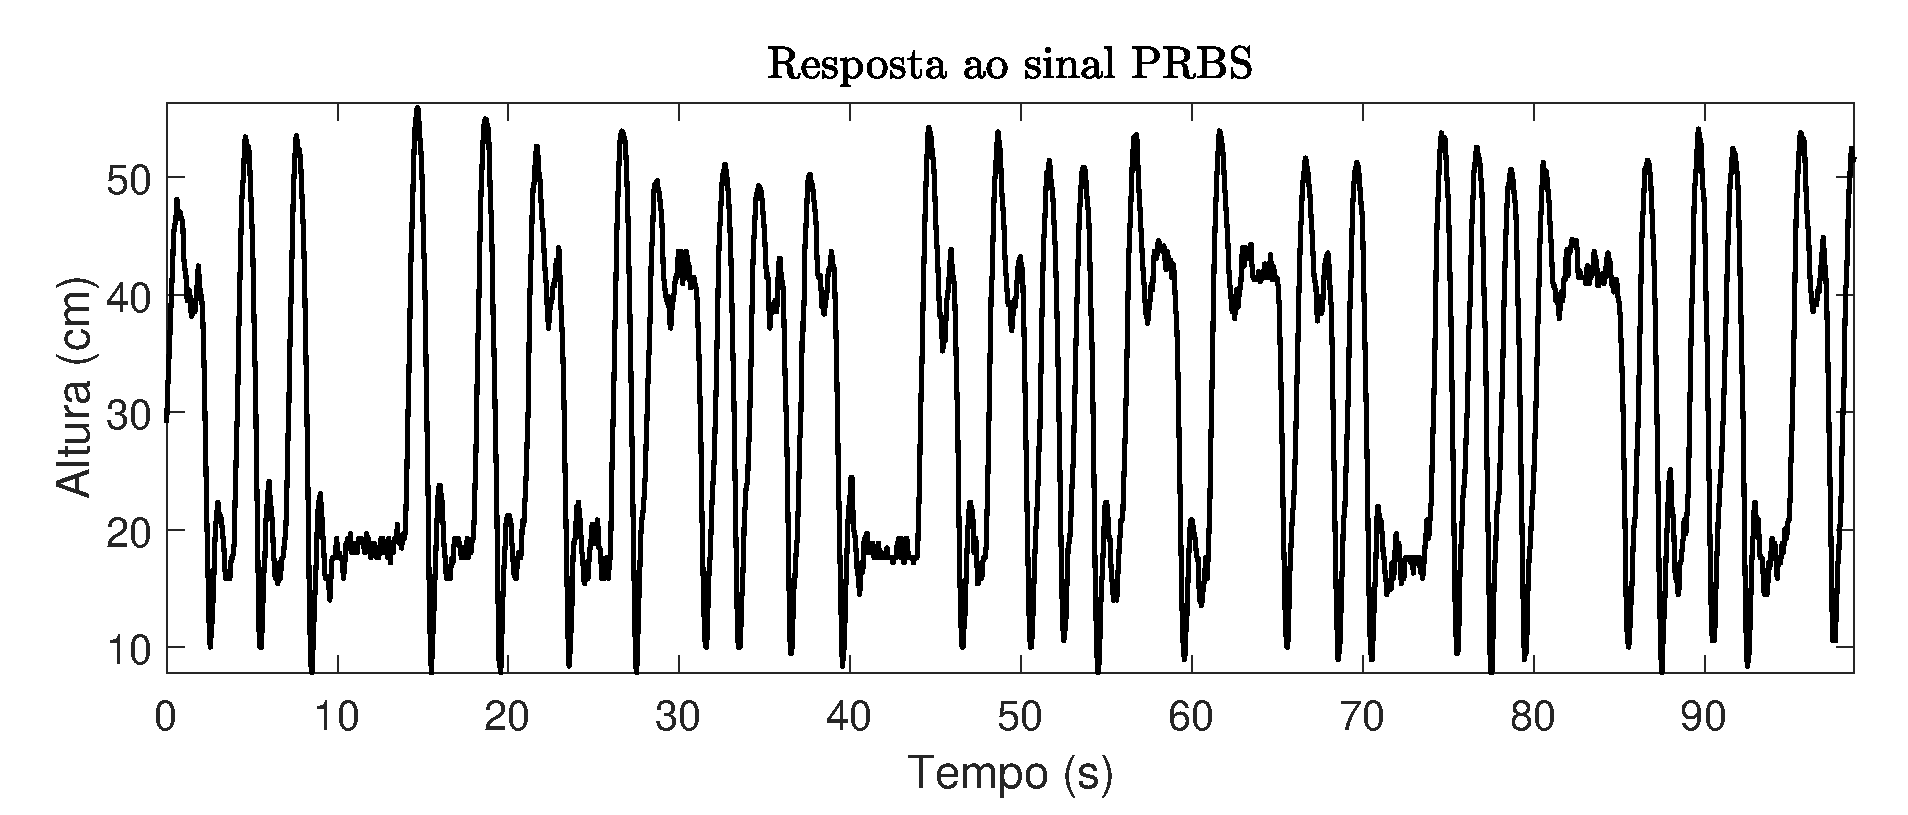
\includegraphics[width=1\linewidth]{sinalprbsid}
	\caption[Gráfico da saída PRBS do sistema]{Gráfico da saída do sistema ao aplicar o sinal PRBS com tempo de amostragem de 50 ms}
	\label{fig:sinalprbsid}
\end{figure}

\begin{figure}[H]
	\centering
	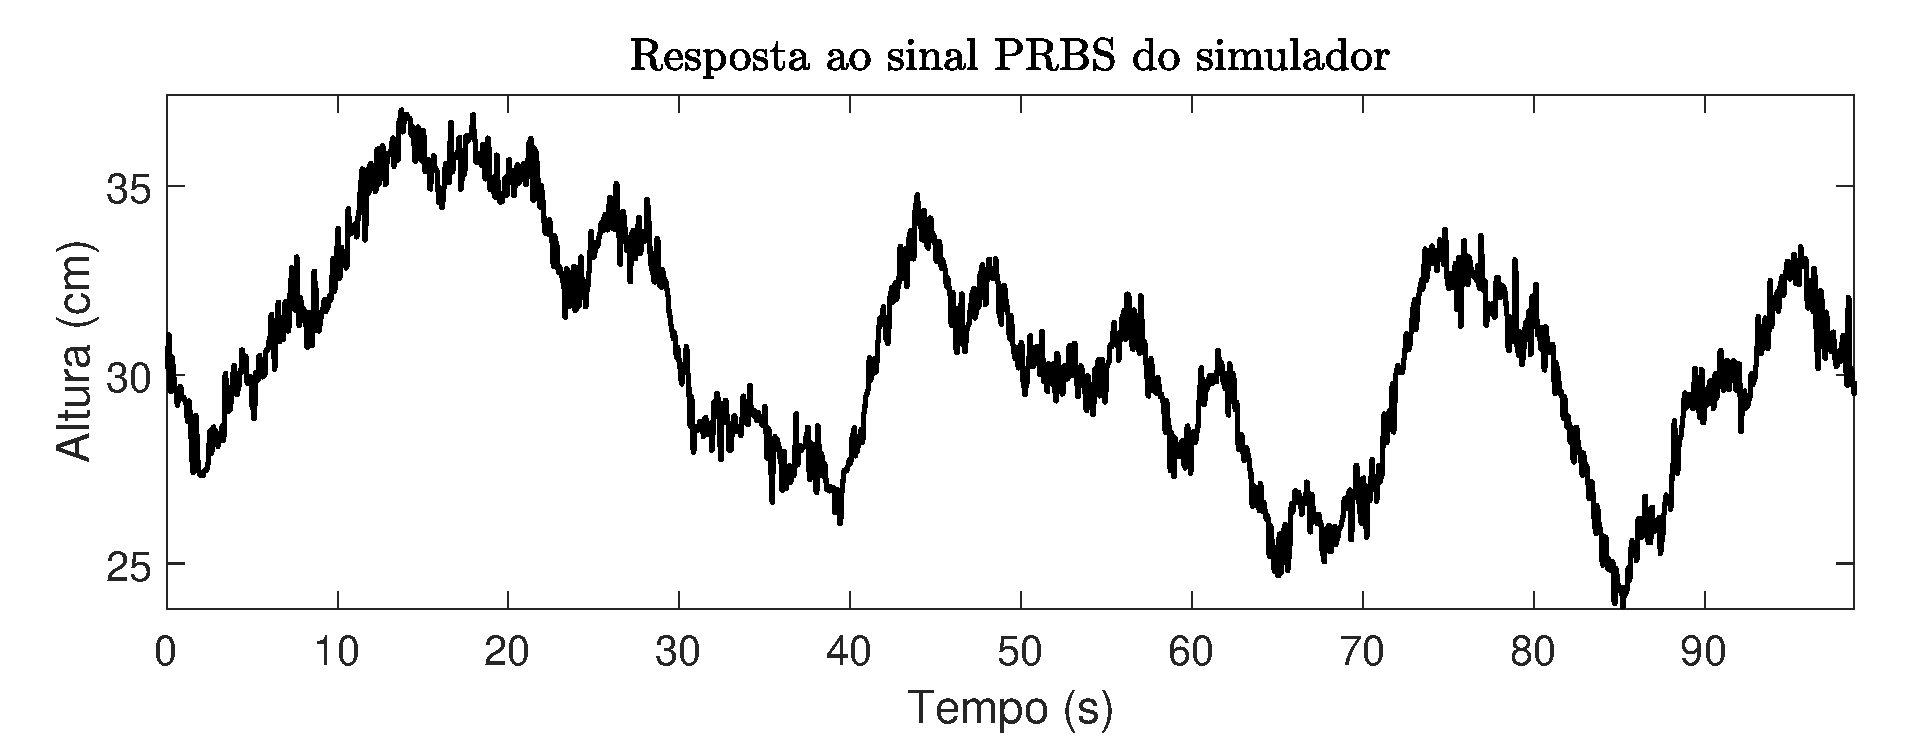
\includegraphics[width=1\linewidth]{sinalprbsidsimul}
	\caption[Gráfico da saída PRBS do simulador]{Gráfico da saída do simulador ao aplicar o sinal PRBS com tempo de amostragem de 50 ms}
	\label{fig:sinalprbsidsimul}
\end{figure}


A figura \ref{fig:sinalprbsid} mostra a resposta do sistema ao sinal PRBS que foi aplicado ao sistema, e a figura \ref{fig:sinalprbsidsimul} mostra a resposta do simulador. Vemos que a resposta do modelo simulado é muito diferente do sistema real.

\section{Estimação}\label{s:4estimacao}

Com a resposta ao sinal PRBS em mãos podemos identificar o sistema. Usando o método dos mínimos quadrados e o método de identificação por subespaços.

\subsection{Mínimos Quadrados}\label{s:4estmq}
Para fazer a identificação por mínimos quadrados geramos a matriz de regressores $\psi$ da equação \eqref{eq:regressores} e usamos a equação \eqref{eq:MQ} para obter os coeficientes dos regressores. Obtemos o coeficientes do modelo $ARX1$:

\begin{equation}
\begin{matrix}
a_1= 0.0017 &
a_2=0.0011&
a_3=0.0550
\end{matrix}
\end{equation}
\begin{equation}
\begin{matrix}
b_1= -1.6309   &
b_2= 0.5828 &
b_3=   0.0965
\end{matrix}
\end{equation}

Obtemos os coeficientes do modelo $ARX2$:
\begin{equation}
\begin{matrix}
a_1= -0.0029  &
a_2= -0.0040   &
a_3= 0.0143  &
a_4=  0.0057 &
a_5=  0.0725
\end{matrix}
\end{equation}
\begin{equation}
\begin{matrix}
b_1= -1.5506  &
b_2=  0.7601  &
b_3= -0.5321  &
b_4=  0.4854 &
b_5=  -0.0897
\end{matrix}
\end{equation}

Obtemos os coeficientes do modelo $ARXsim$:

\begin{equation}
\begin{matrix}
a_1= -0.0037 &
a_2=  0.0017 &
a_3=   0.0066 
\end{matrix}
\end{equation}
\begin{equation}
\begin{matrix}
b_1=-1.0108   &
b_2= 0.4531  &
b_3= -0.4341
\end{matrix}
\end{equation}


\subsection{Subespaços}\label{s:4estsub}

Para identificar o sistema usando subespaços utilizamos o algoritmo mostrado na seção \ref{s:subalgoritmos} com uma matriz em blocos de Hankel de ordem 15 para encontrar um sistema de ordem 3. Identificamos o seguinte modelo, $SUB1$, com o formato da equação \eqref{eq:ss}:

\begin{equation}
A=\begin{bmatrix}
0.9761  &  0.1933 &  -0.0438\\
-0.1817  &  0.9841  & -0.1489\\
0.0840  &  0.3107  &  0.6994
\end{bmatrix}
\end{equation}

\begin{equation}
B=\begin{bmatrix}
0.1466\\
0.2515\\
0.8460
\end{bmatrix}
\end{equation}
\begin{equation}
C=\begin{bmatrix}
-1.0104 &  -0.3354 &   0.2496
\end{bmatrix}
\end{equation}
\begin{equation}
D=\begin{bmatrix}
0.0010
\end{bmatrix}
\end{equation}

\section{Validação}\label{s4:val}
Ao identificar um sistema precisamos validar o modelo obtido para garantir que ele é adequado para representar o sistema real. Para isso fazemos uma análise da auto correlação dos resíduos $\xi=y-\Psi \hat{\theta}$ para o ARX e $\xi=y-y_{sim}$ para o espaço de estados. Vemos nas figuras \ref{fig:autocorrelacaoARX1}, \ref{fig:autocorrelacaoARX2} e \ref{fig:autocorrelacaosub1}, que os resíduos do modelo ARX são muito menos correlacionados do que os do modelo em espaço de estados. Isso acontece porque para o modelo ARX estamos analisando os seus regressores com a matriz $\Psi$ que os gera, o que retorna uma resposta muito mais próxima do sistema. Já para o espaço de estados estamos analisando a simulação do sistema, que apresenta pequenas diferenças em relação ao sistema real, como a ausência de ruído.


Olhamos também a resposta ao degrau do sistema, figuras \ref{fig:respostadegrauarx1}, \ref{fig:respostadegrauarx2}, \ref{fig:respostadegrauarxsim} e  \ref{fig:respostadegrausub}, e vemos que para os dois sistemas identificados ela tem uma oscilação similar ao sistema real. Concluímos, através da análise da auto correlação dos resíduos e da análise da resposta ao degrau dos sistemas identificados, que os modelos são adequados para mostrar o funcionamento do sistema.

\begin{figure}[H]
	\centering
	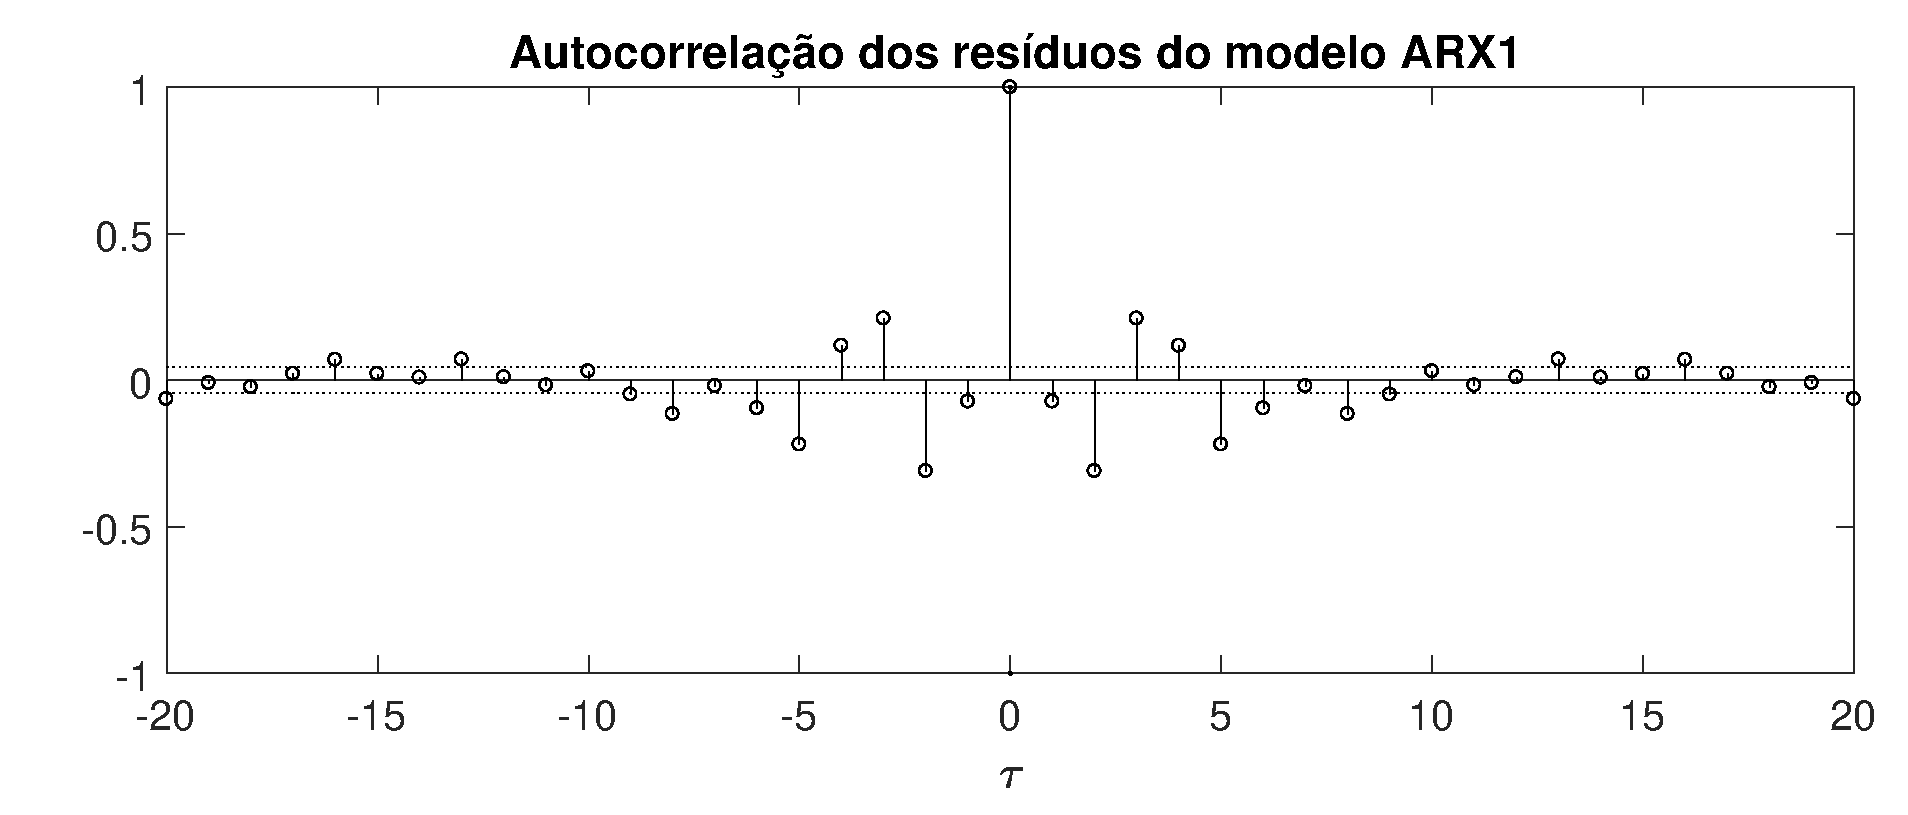
\includegraphics[width=1\linewidth]{autocorrelacaoARX1}
	\caption[Autocorrelação dos resíduos do modelo $ARX1$]{Autocorrelação dos resíduos do modelo $ARX1$}
	\label{fig:autocorrelacaoARX1}
\end{figure}

\begin{figure}[H]
	\centering
	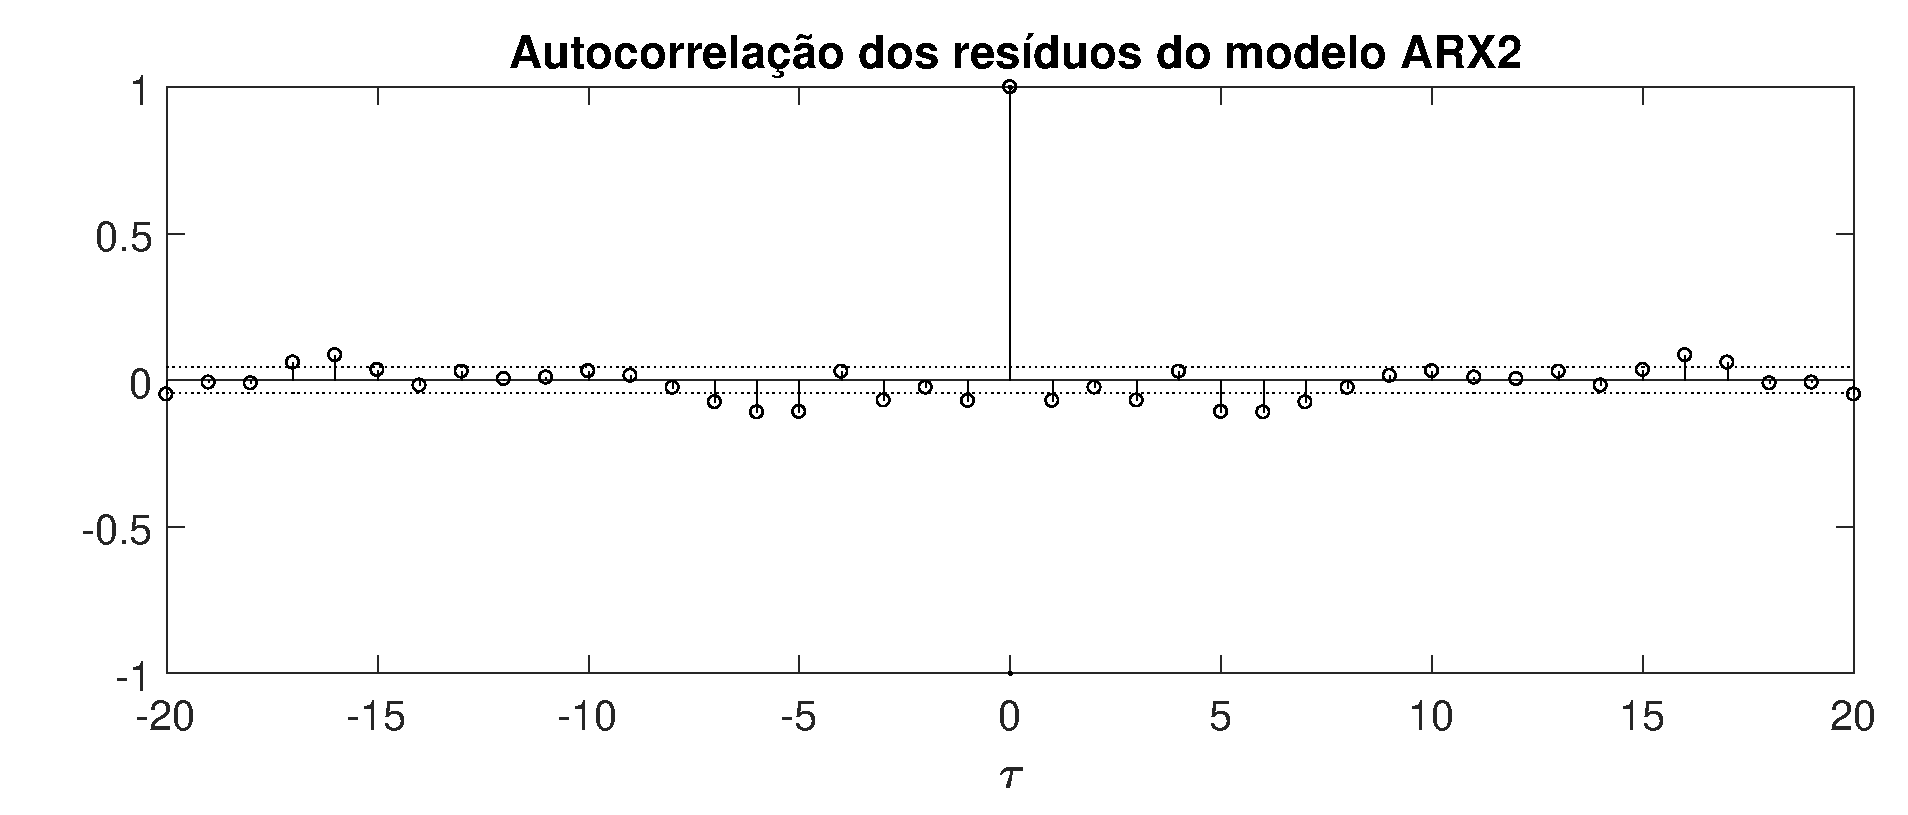
\includegraphics[width=1\linewidth]{autocorrelacaoARX2}
	\caption[Autocorrelação dos resíduos do modelo $ARX2$]{Autocorrelação dos resíduos do modelo $ARX2$}
	\label{fig:autocorrelacaoARX2}
\end{figure}

\begin{figure}[H]
	\centering
	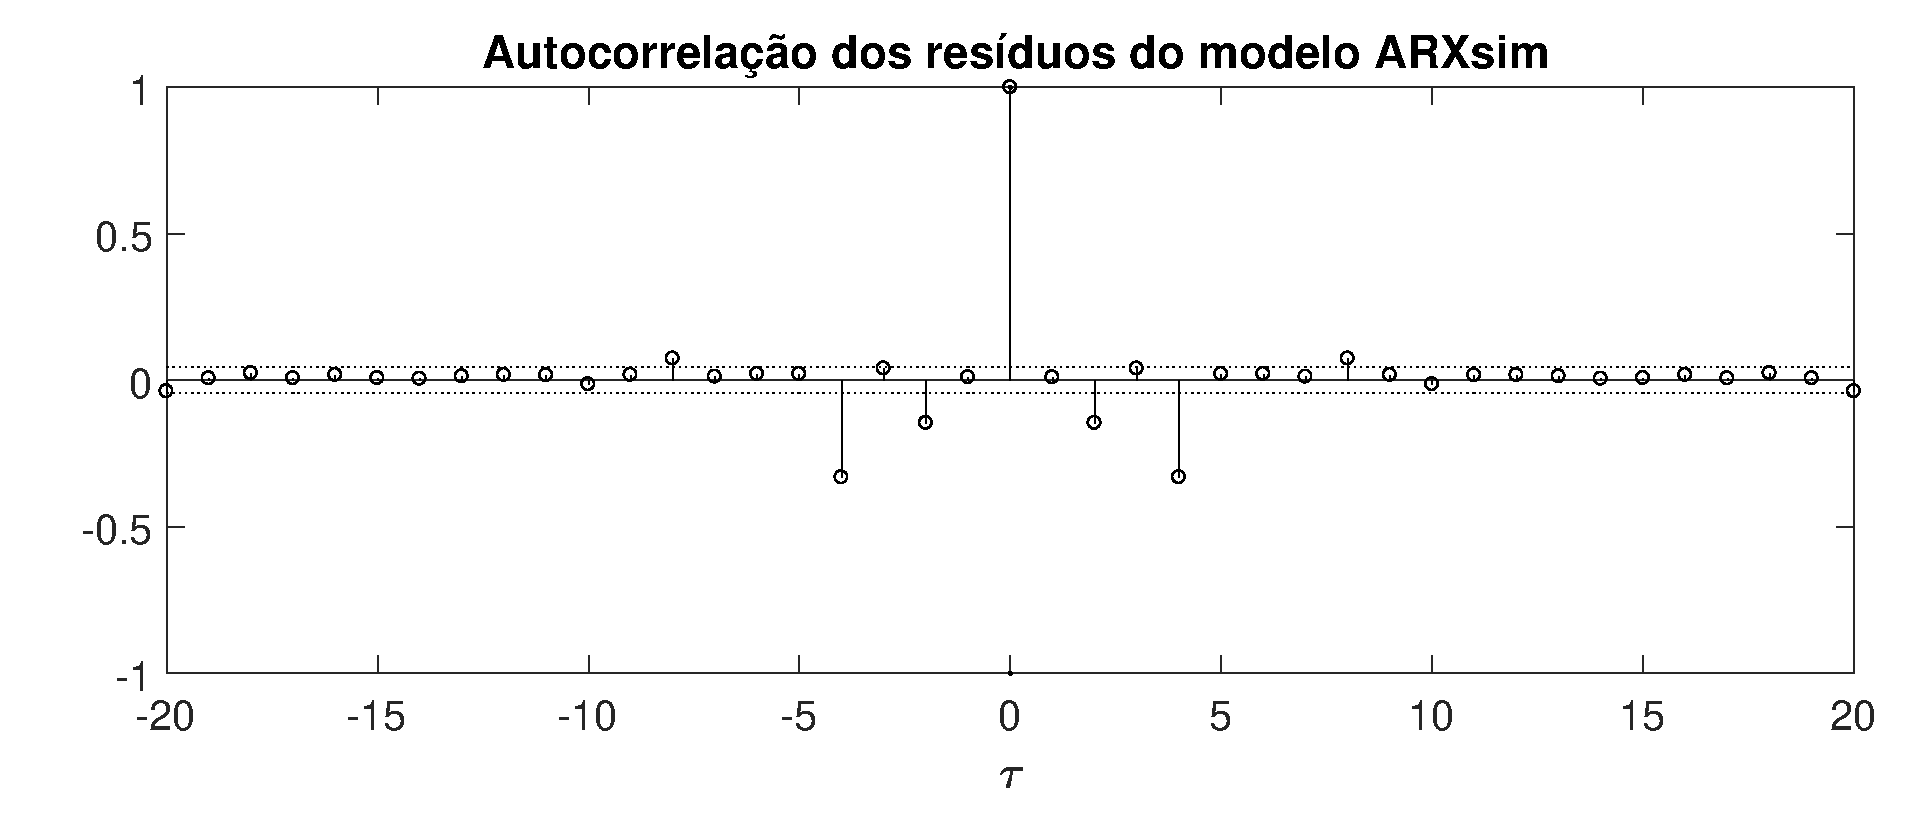
\includegraphics[width=1\linewidth]{autocorrelacaoARXsim}
	\caption[Autocorrelação dos resíduos do modelo $ARXsim$]{Autocorrelação dos resíduos do modelo $ARXsim$}
	\label{fig:autocorrelacaoarxsim}
\end{figure}

\begin{figure}[H]
	\centering
	\includegraphics[width=1\linewidth]{autocorrelacaosub1}
	\caption[Autocorrelação dos resíduos do modelo $SUB1$]{Autocorrelação dos resíduos do modelo $SUB1$}
	\label{fig:autocorrelacaosub1}
\end{figure}

\begin{figure}[H]
	\centering
	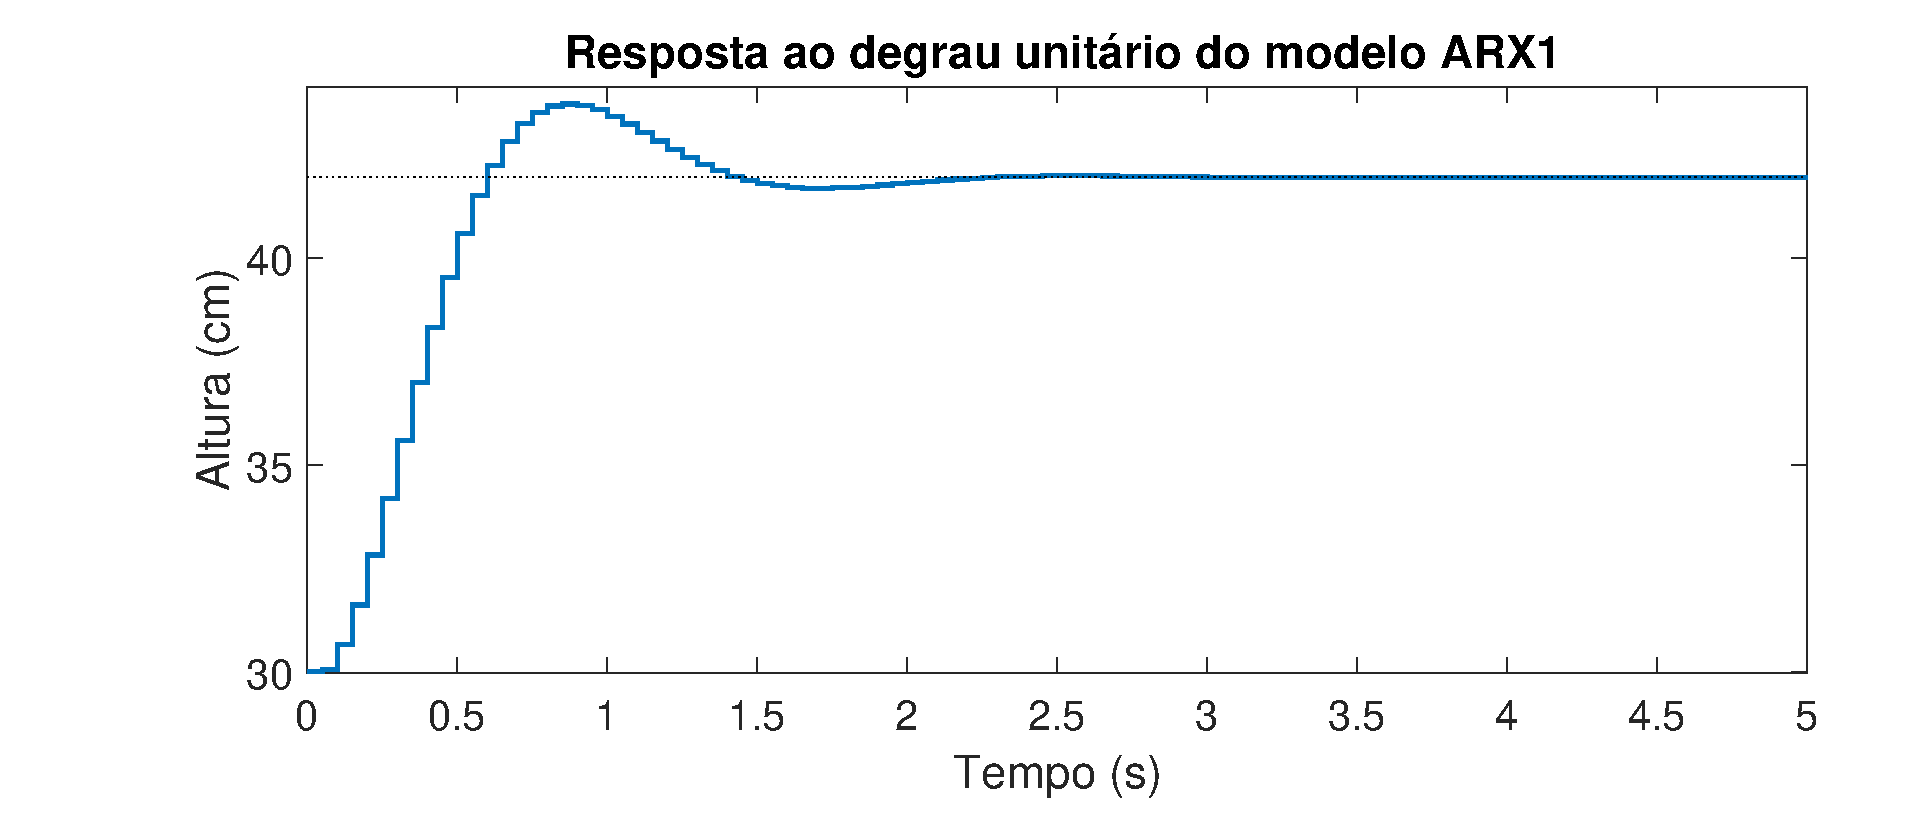
\includegraphics[width=1\linewidth]{respostadegrauarx1}
	\caption[Resposta ao degrau do modelo $ARX1$]{Resposta ao degrau unitário do modelo $ARX1$}
	\label{fig:respostadegrauarx1}
\end{figure}

\begin{figure}[H]
	\centering
	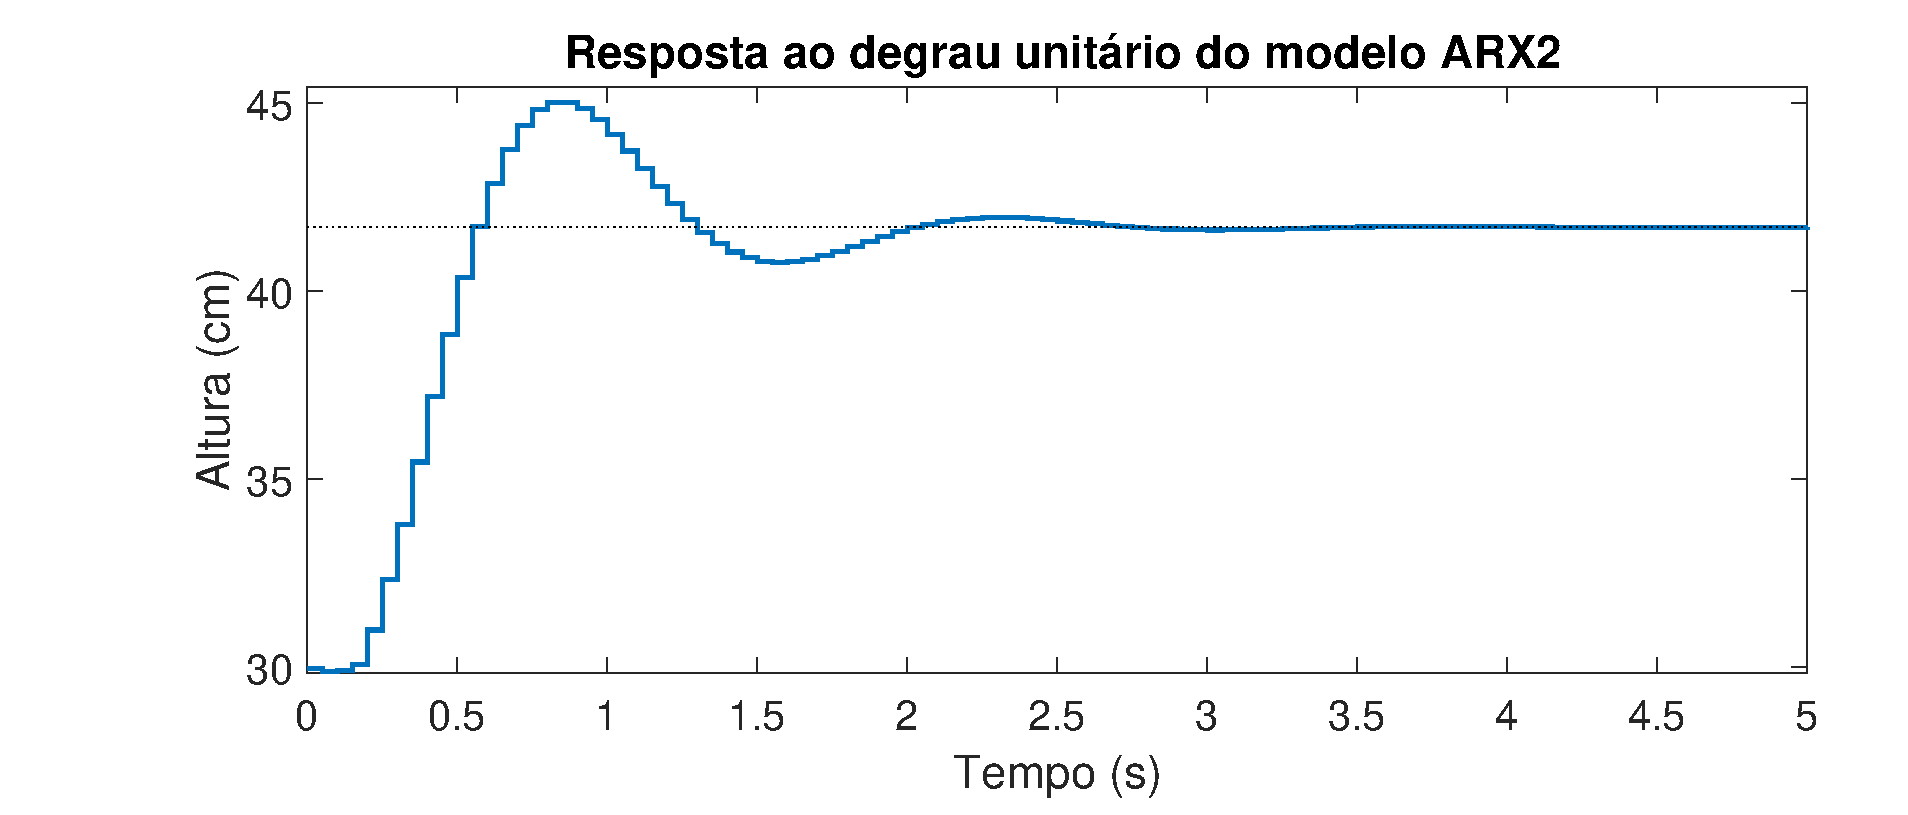
\includegraphics[width=1\linewidth]{respostadegrauarx2}
	\caption[Resposta ao degrau do modelo $ARX2$]{Resposta ao degrau unitário do modelo $ARX2$}
	\label{fig:respostadegrauarx2}
\end{figure}

\begin{figure}[H]
	\centering
	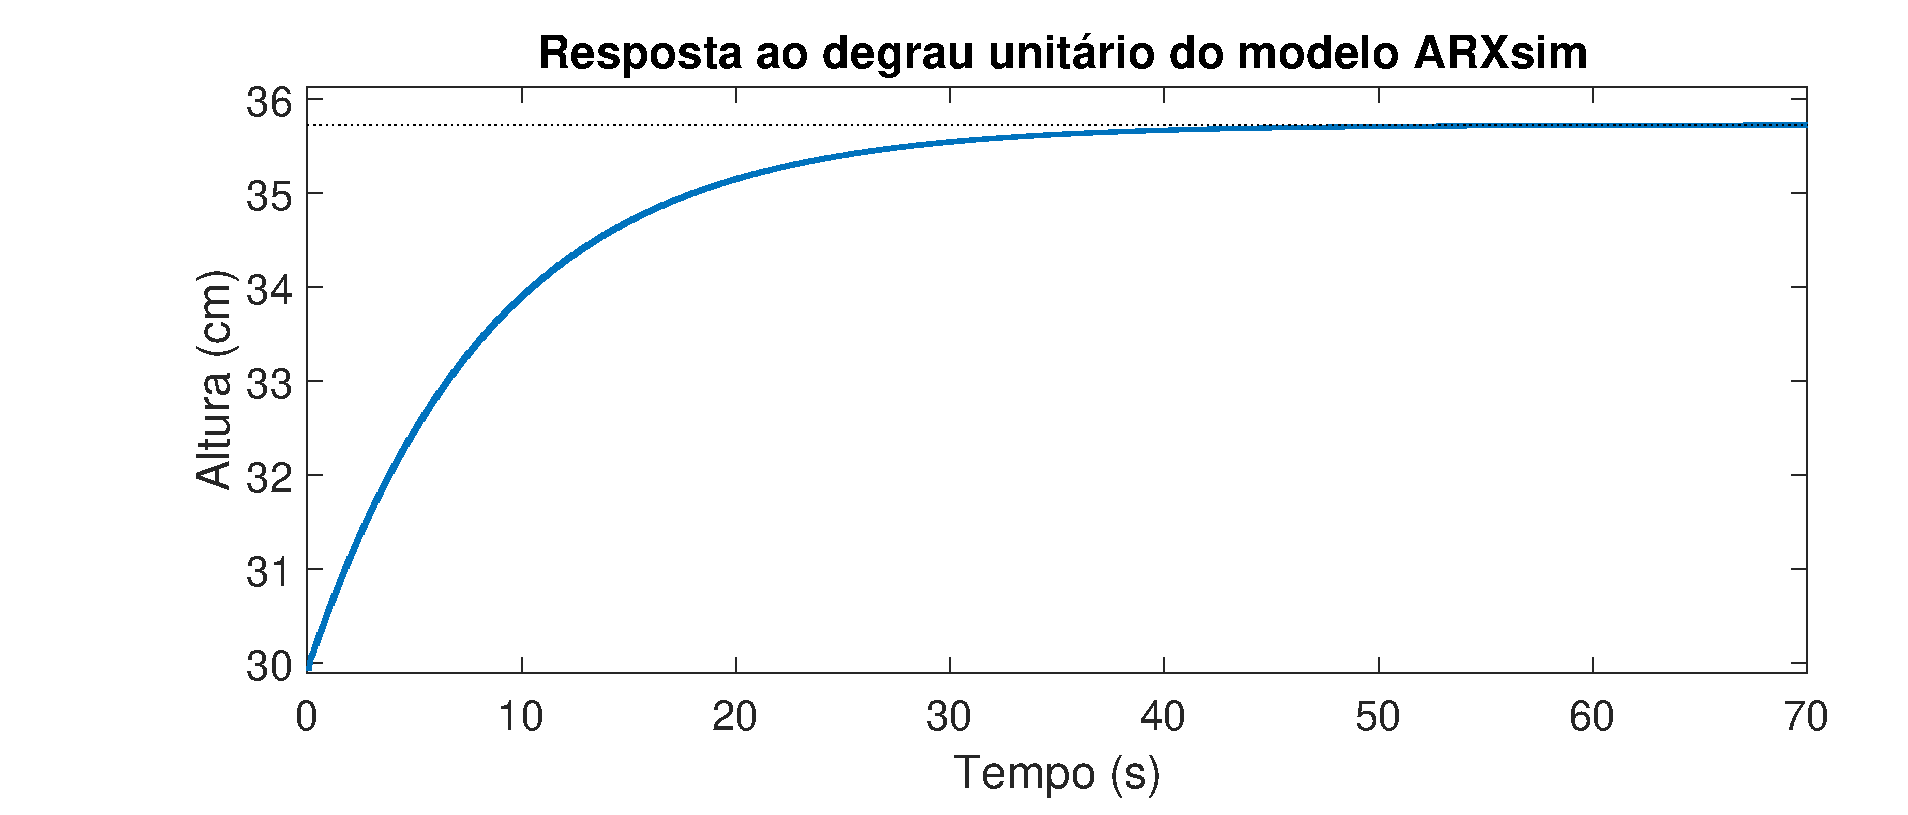
\includegraphics[width=1\linewidth]{respostadegrauarxsim}
	\caption[Resposta ao degrau do modelo $ARXsim$]{Resposta ao degrau unitário do modelo $ARXsim$}
	\label{fig:respostadegrauarxsim}
\end{figure}

\begin{figure}[H]
	\centering
	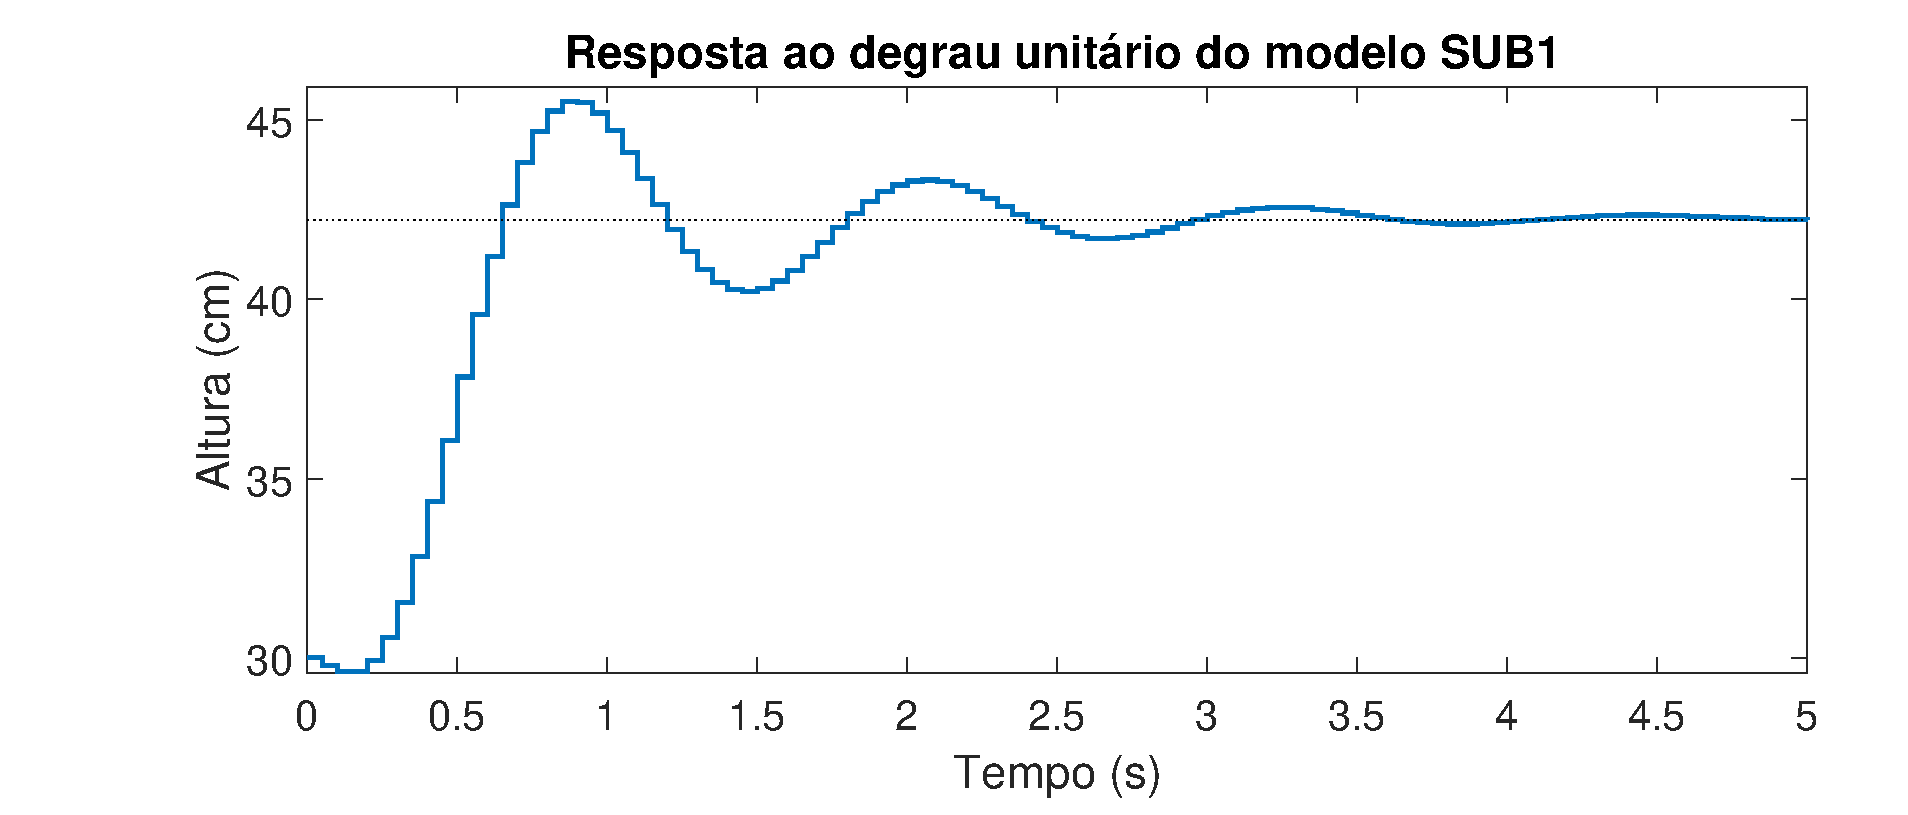
\includegraphics[width=1\linewidth]{respostadegrausub1}
	\caption[Resposta ao degrau do modelo $SUB1$]{Resposta ao degrau unitário do modelo $SUB1$}
	\label{fig:respostadegrausub}
\end{figure}

\commentib{Você precisa discutir esse bando de figuras.... Além disso, seria interesante comparar os desempenhos dos modelos identificados com os sistemas identificados}

% Fim Capítulo